\documentclass{beamer}
\usepackage{listings}
\usetheme{Copenhagen}
\usecolortheme{beaver}
\setbeamertemplate{navigation symbols}{}
\setbeamertemplate{footline}{\parbox[t][12pt][c]{12pt}{~\scriptsize\insertframenumber}}
% \usepackage{beamerthemesplit} // Activate for custom appearance

\title{Declarative Cartography}
\subtitle{In-Database Map Generalization of Spatial Datasets}
\author{Pimin Konstantin Kefaloukos, Marcos Vaz Salles, Martin Zachariasen}
\date{\today}

\begin{document}

\frame{\titlepage}

% MOTIVATION
\frame
{
  \frametitle{Goals for project}
  \begin{itemize}
  \item \textbf{Language}: Design and implement an easy to use \emph{programming language} for generalizing (\emph{selection}) spatial data 
  \item \textbf{Optimization}: Fit generalization problem to well-known \emph{optimization problem} (set multi-cover problem~\cite{vazirani}) and \emph{reuse existing algorithms}: Solve a \emph{global} optimization problem
  \item \textbf{DB-technology}: Compute solution by using a \emph{spatial database as the runtime} (moving code to data + scalability)
  \end{itemize}
  \begin{center}
  \fbox{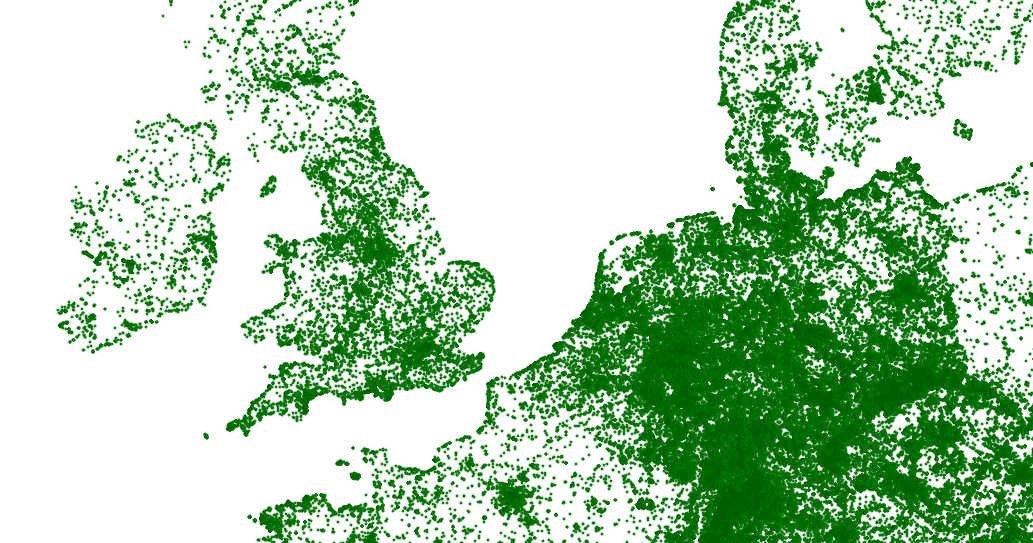
\includegraphics[scale=0.20]{figs/toomanyobjects.png}}
  \end{center}
}

\frame
{
  \frametitle{Reverse data management}
  Implement \emph{how-to} queries for spatial data:
  \begin{itemize}
  \item \textbf{How-to queries}~\cite{reversedatamanagement}: Given an input database; compute an output database subject to set of \emph{constraints} and an \emph{objective function}
  \item \textbf{Example}: given a database table representing a stock portfolio, compute a new stock portfolio table that has $10\%$ higher yield while minimizing number of stock sales and acquisitions.
  \item \textbf{Spatial example}: Given an input database of spatial objects; compute an output database that generalizes the objects to $\mathcal{Z}$ zoom-levels
  \end{itemize}
}

\frame
{
  \frametitle{Problem definition}
  \begin{itemize}
  \item Given a database of spatial objects, each having a \emph{unique ID} and a \emph{geometry} (point, linestring, polygon etc)
  \item Compute for each object the minimum zoom-level where it becomes visible (optimizing an \emph{objective} and respecting some \emph{constraints})
  \end{itemize}
  \begin{center}
  \fbox{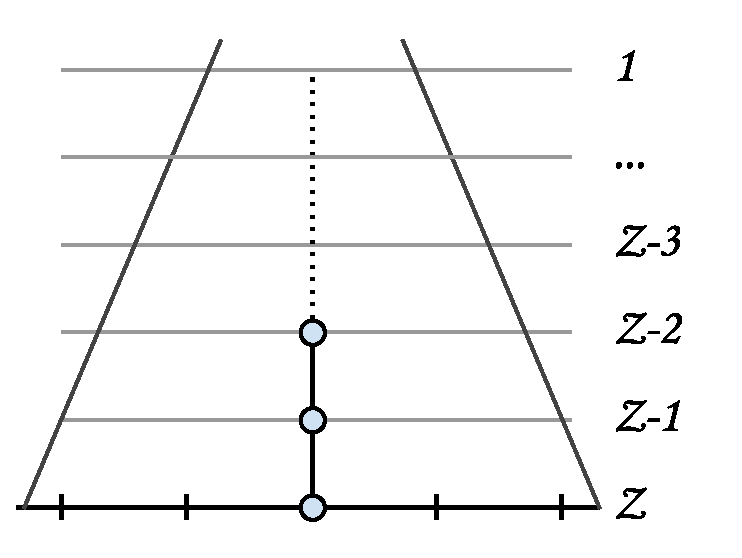
\includegraphics[scale=0.4]{figs/cvl-problem.pdf}}
  \end{center}
}

\frame
{
  \frametitle{Constraints}
  \begin{description}
  \item [Zoom-consistency] As you zoom in, records only appear, never disappear~\cite{fusiontables}
  \item [User-defined constraints] Must fit pattern of finding and resolving \emph{conflicts}, e.g. proximity
  \end{description}
  \begin{center}
  \fbox{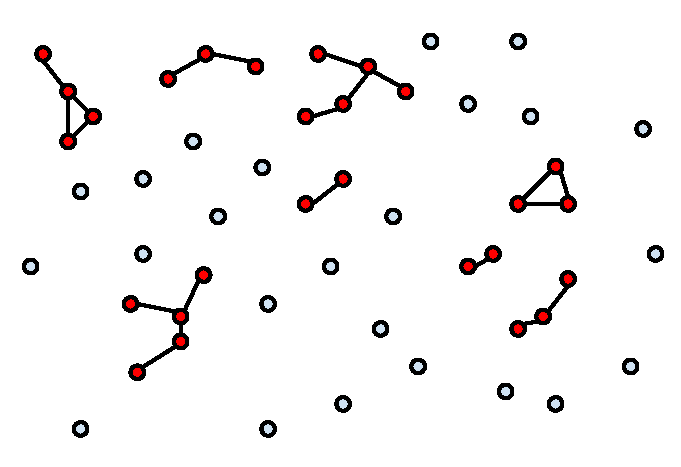
\includegraphics[scale=0.4]{figs/cvl-proximity.pdf}}
  \end{center}
}



\frame
{
  \frametitle{Future work}
  \begin{itemize}
  \item Relax zoom-consistency: \emph{min} and \emph{max} zoom-level for records)
  \item Extend work with \emph{aggregation} in language (semantics) and algorithm (implementation)
  \item Implement compilation of CVL to a distributed database dialect
  \end{itemize}
}


% RELATED WORK
\frame
{
  \frametitle{Related work}

  \begin{itemize}
  \item \emph{Reverse data management}, Meliou, A., Gatterbauer, W., \& Suciu, D. (2011).
  \item \emph{Efficient Spatial Sampling of Large Geographical Tables}. Das Sarma, A., Lee, H., Gonzalez, H., Madhavan, J., \& Halevy, A. (2012).
  \item \emph{Generalization of land cover maps by mixed integer programming}. Haunert, J.-H., \& Wolff, A. (2006). 
  \item \emph{Constant information density in zoomable interfaces}. Woodruff, A., Landay, J., Stonebraker, M. (1998).
  \end{itemize}
}

% Past and future work
\frame
{
  \frametitle{Past and future work}

  \begin{itemize}
  \item Past work: \emph{TileHeat}, predicting where people will look on a map tomorrow
  \item Latest work: \emph{Declarative Cartography}, the work described in these slides
  \item Future work: \emph{Real-time Declarative Cartography}, joint work with people at University of Zurich (Department of Geography)
  \item Future work: Succinct data representation of high-fidelity spatial data that is visualized on a digital map on a screen (think: pixel precision is not all that good)
  \end{itemize}
}




\end{document}
